\section{Q2: CNN versus MLP}
\label{sec:q2}

\subsection{(a) A fair comparison and a proposed reason}
\textbf{Fairness criterion (written down before any test number existed).} The two models are the Q1(a) MLP
(1{,}150{,}474 parameters) and CNN (1{,}148{,}874), reused from Q1. They are compared at matched parameter
count and matched training budget: the same 45k images, 40 epochs, optimiser, schedule, batch size, weight
decay, seed and BatchNorm/ReLU; the same learning-rate grid with selection on validation; and no augmentation
for either, because flips and crops assume an intact spatial layout and would not be the same treatment once the
pixels are permuted in (b). Computation per step is not matched (see Q1). Each model is tested once after
selection.

\textbf{Proposed reason (also stated beforehand).} The CNN's advantage comes from exploiting the local spatial
arrangement of pixels: neighbouring pixels are strongly correlated and the same local pattern can occur
anywhere, which local receptive fields and weight sharing~\cite{lecun1998gradient} use directly. The MLP has no
access to this arrangement.

\begin{table}[t]
\centering
\small
\begin{tabular}{@{}lcccc@{}}
\toprule
& \multicolumn{2}{c}{MLP (1{,}150{,}474)} & \multicolumn{2}{c}{CNN (1{,}148{,}874)} \\
\cmidrule(lr){2-3}\cmidrule(l){4-5}
Condition & lr & Test & lr & Test \\
\midrule
Clean (Q1(a) runs) & 0.3 & 0.573 & 0.3 & \textbf{0.897} \\
Pixel permutation & 0.3 & 0.576 & 0.3 & 0.561 \\
$16\times16$ patches shuffled & 0.3 & 0.403 & 0.3$^*$ & 0.815 \\
$8\times8$ patches shuffled & 1.0 & 0.324 & 0.3 & 0.705 \\
$4\times4$ patches shuffled & 1.0 & 0.276 & 0.3$^*$ & 0.602 \\
\bottomrule
\end{tabular}
\caption{Q2. Compared models with parameter counts and test accuracy under each condition (train and test use
the same transformation). $^*$CNN learning rate taken from the $8\times8$ validation result; all others chosen
on validation from the full grid.}
\label{tab:q2}
\end{table}

\begin{figure}[t]
\centering
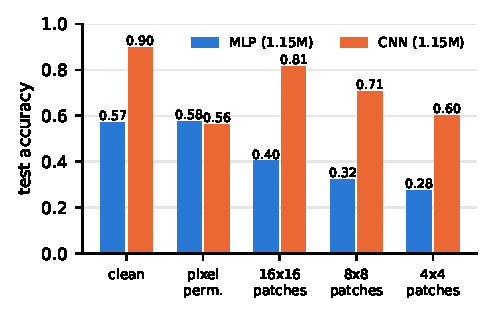
\includegraphics[width=\columnwidth]{q2_accuracy_by_condition}
\caption{Q2. Test accuracy of the MLP and CNN under the clean, permuted and patch-shuffled conditions.}
\label{fig:q2acc}
\end{figure}

\textbf{Result.} Under this criterion the CNN reaches 0.897 and the MLP 0.573 on test (Tab.~\ref{tab:q2}), a gap
of 32.4 points that can only come from how the same number of parameters is wired.

\subsection{(b) Same pixels, disturbed spatial structure}
\textbf{Transformation.} One fixed random permutation of the 1024 pixel positions (seed 242003), applied
identically to the three colour channels and to every training, validation and test image. Pixel values are
unchanged and the mapping is the same for every image, so all information is still present; only the
neighbourhood structure is gone. Both models were retrained from scratch with the same protocol and grid.

\textbf{Prediction (stated before running).} The MLP should not change beyond noise (about one point): a fixed
permutation of its inputs is equivalent to permuting the rows of its first weight matrix, so the function class
is identical and only the initialisation and batch order differ. The CNN should drop to roughly the MLP level or
below, since its $3\times3$ filters and pooling now combine pixels that are not neighbours. If the CNN kept most of
its advantage, the reason proposed in (a) would be wrong.

\textbf{Result.} Both predictions hold (Tab.~\ref{tab:q2}, Fig.~\ref{fig:q2acc}). The MLP moves from 0.573 to
0.576, within noise. The CNN falls from 0.897 to 0.561, slightly \emph{below} the permuted MLP, although every
pixel value is still available. Destroying neighbourhoods removes the CNN's entire advantage, which supports the
reason proposed in (a); with the arrangement gone, its local filters even work slightly against it.

\subsection{(c) Local evidence or global layout?}
Two explanations for what the CNN uses remain after (b): (A) \emph{local evidence}, i.e.\ textures, colours and
small parts within small windows (a ``bag of local features''~\cite{brendel2019bagnet}), or (B) the \emph{global
layout} of those parts, i.e.\ object shape and configuration. Both need intact neighbourhoods, so (b) cannot tell
them apart. We cut each image into a grid of $p\times p$ patches and put the patches back in a random order that
is different for every image (fixed seeds per split, the same procedure for train, validation and test). Inside a
patch everything is intact; between patches the arrangement is destroyed. If (A) holds, accuracy should stay high
once patches are big enough to contain a recognisable part; if (B) matters, it should drop strongly even for large
patches. We use $p=8$ as the main condition (both models, full learning-rate grid) and $p=4$ and $p=16$ as a
sweep (CNN learning rate taken from the $p=8$ validation result; MLP full grid). Errors and confidence are
analysed on test.

\begin{figure*}[t]
\centering
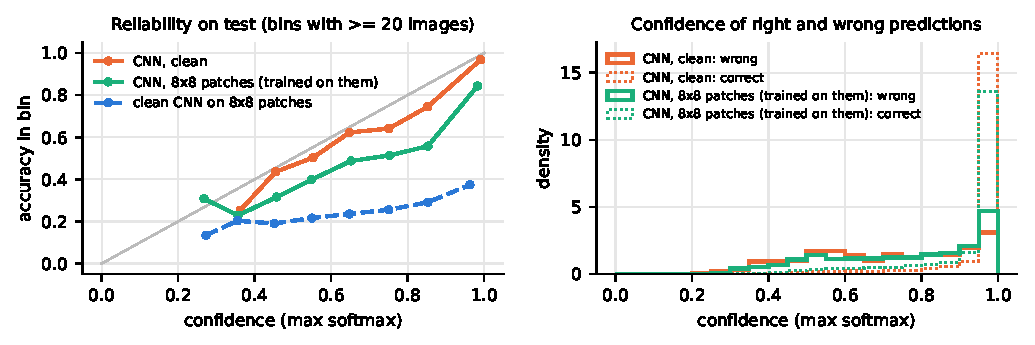
\includegraphics[width=\textwidth]{q2_confidence}
\caption{Q2(c), test set. Left: reliability of the clean CNN, the CNN trained and tested on $8\times8$ shuffles,
and the clean CNN tested on $8\times8$ shuffles. Right: confidence of correct (dotted) and wrong (solid)
predictions.}
\label{fig:q2conf}
\end{figure*}

\begin{table}[t]
\centering
\small
\begin{tabular}{@{}lccccc@{}}
\toprule
CNN, test & Acc. & Conf.\ right & Conf.\ wrong & Wrong $>0.9$ & ECE \\
\midrule
Clean & 0.897 & 0.956 & 0.710 & 25\% & 0.033 \\
$16\times16$ & 0.815 & 0.938 & 0.730 & 28\% & 0.085 \\
$8\times8$ & 0.705 & 0.919 & 0.753 & 34\% & 0.164 \\
$4\times4$ & 0.602 & 0.894 & 0.753 & 33\% & 0.236 \\
Clean model on $8\times8$ & 0.277 & 0.781 & 0.707 & 27\% & 0.450 \\
\bottomrule
\end{tabular}
\caption{Q2(c). Mean max-softmax confidence of right and wrong predictions, share of errors made with
confidence above 0.9, and expected calibration error (15 bins)~\cite{guo2017calibration}.}
\label{tab:q2conf}
\end{table}

\textbf{Accuracy.} Accuracy falls gradually as patches shrink: 0.897 (intact), 0.815 ($p=16$), 0.705 ($p=8$),
0.602 ($p=4$) and 0.561 for single pixels (the permutation of (b)). With $8\times8$ patches in a random order the
CNN keeps 79\% of its clean accuracy and stays 38 points above the MLP under the same shuffle, so local evidence
(A) carries most of its performance. The MLP collapses (0.573 to 0.324) because its weights are tied to absolute
positions. Layout (B) is not irrelevant: shuffling $8\times8$ patches still costs the CNN 19 points.

\textbf{Errors.} The loss is not uniform. Per-class recall drops most for cat ($-27$), deer ($-26$), bird
($-22$), horse ($-22$) and dog ($-21$) and least for ship ($-10$) and truck ($-14$). The confusions that grow are
between classes that share texture and colour and differ mainly in shape: dog$\to$cat 89$\to$178,
cat$\to$dog 76$\to$175, automobile$\to$truck 34$\to$108, deer$\to$frog 15$\to$93. Classes with distinctive
local context (water around ships, frog skin texture) survive.

\textbf{Confidence.} The clean CNN is well calibrated (ECE 0.033, Tab.~\ref{tab:q2conf}, Fig.~\ref{fig:q2conf}).
Without layout the CNN does not become uncertain: its confidence on \emph{wrong} predictions rises (0.710 to
0.753) and 34\% of its errors are made with more than 0.9 confidence. It decides confidently from local evidence
and is simply wrong more often, which is what a bag-of-local-features decision would do. As a side check, the
clean-trained CNN applied to $8\times8$-shuffled test images (not a train=test condition) drops to 0.277 at 0.73
mean confidence: trained on intact images it does use the layout it is given.

\textbf{Conclusion linking (a)--(c).} The CNN wins by 32 points at equal budget (a). Removing pixel
neighbourhoods removes the whole gain, so the gain comes from spatial arrangement (b). Of that arrangement, local
neighbourhoods carry most of the accuracy, and global layout contributes a smaller part concentrated in classes
that look alike locally (c).
